\section{Experiments and Discussion}
\label{sec:HomographyExperiments}

\figstr{}~\ref{fig:HeatmapsBestWorst} demonstrates how the reprojection error varies with respect to the marker position. It can be observed that the marker position can be approximately estimated by looking at the heatmap which represents the pixel-wise reprojection error over the image. Simply put, the transformation achieves the best accuracy in the vicinity of the chosen marker and steadily decreases for more distant pixels. However, the important property is that not all markers are subjected to the same pattern of error variation. This is the core observation that motivated our solution in the first place. The objective is to select the marker that minimizes the pixel-wise reprojection error within the region of the image that is as broad as possible. That is why we evaluate our method by computing the reprojection error over each pixel, not just the keypoints. The rationale is that subsequent image postprocessing would greatly benefit from having the area of the image as large as possible that is reprojected properly.

% ------------------------------------------------------------------------------
\begin{figure}[t]
    \centerline{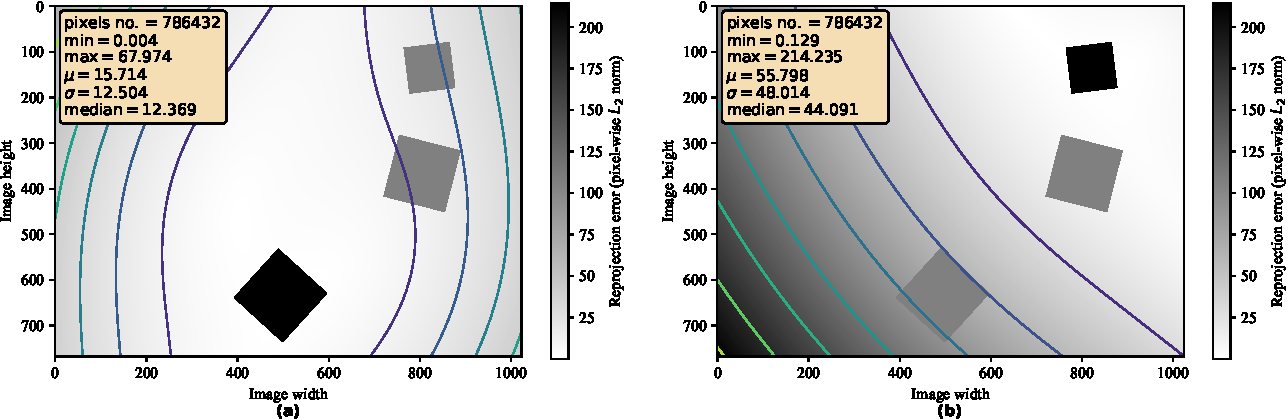
\includegraphics[width=\linewidth]{figures/homography/heatmaps_best_worst.pdf}}
    \caption[Homography ranking heatmaps]{Distribution of pixel-wise reprojection error. The heat map along with the corresponding contours demonstrate the varying distance between the ground truth and rectified pixel position after removing the perspective distortion. The bold square represents the reference marker. We show the result of \imgpartdesc{a} the ``best'' marker and \imgpartdesc{b} the ``worst'' marker. This test scenario includes all similarity transformations as well as noise in point correspondence.}
    \label{fig:HeatmapsBestWorst}
\end{figure}
% ------------------------------------------------------------------------------

The evaluation of the proposed homography ranking algorithm involved various conditions. We tested cases that included diverse similarity transformations applied to original markers as well as noisy point correspondence, e.g., errors in marker detection since these are the expected problems in real-world scenarios.

All the test scenarios indicated the following trend. On average, the homography with the highest score improved the relative performance to the baseline performance the most (both median and mean above $60$\%). The lowest-ranked homography often led to significantly worse performance (median and mean around $-90$\%). These values varied moderately across different setups. The change of shape and number of markers had the greatest impact.

\subsubsection{Implementation Details}
\label{sssec:HomographyImplementation}

Our proposed algorithm can be utilized to extend any homography estimation method that exploits point correspondences. To demonstrate, we adopted time-tested implementations from the OpenCV~$4.4.0$ library~\cite{bradski2008learning}. Each homography was estimated by the \srcfuncname{findHomography} function which internally employs DLT~\cite{abdel2015direct} algorithm for $k = 4$ and RANSAC~\cite{fischler1981ransac} algorithm for $k > 4$, where $k$ is the size of the point correspondences set. At the same time, each optimal similarity transformation between two $2$D point sets was estimated by the \srcfuncname{estimateAffinePartial2D}, which also utilizes RANSAC for robustness. We used the default parameters whenever possible.

% ##############################################################################
\subsection{Dataset Creation}
\label{ssec:HomographyDatasetCreation}

Our synthetic dataset was created to simulate the presence of markers in the scene subjected to perspective distortion. Our experiments were based on a pixel-wise comparison of the reprojection error. This dataset covered multiple setups named as \mbox{\textbf{test scenarios}}. For each test scenario, we generated $t$ different samples which we call \mbox{\textbf{test instances}}. We set $t = 1\ 000$. \tablestr{}~\ref{tab:TestScenariosResults} contains description of the generated test scenarios. To create test instances (within test scenarios), we employed the procedures described below (see \figstr{}~\ref{fig:DatasetGenerating}).

Our dataset easily allows complete reproducibility of the reported results. Thanks to the synthetic nature of our data, fixing the seed for the used pseudo-random generator was sufficient. The source code for running the experiments is freely available on our Github repository~\cite{webhomographyrankinggithub}.

\subsubsection{Image Initialization}

Each test instance was initialized as a blank $1024 \times 768$ image. This image served for $m$ randomly generated copies of the same shape (marker) placed in a $3 \times 3$ grid, where $0 < m \leq 9$. We used a uniform border with $20$\% size of the corresponding side to prevent the generated shapes from reaching outside of the image. We experimented with a different number of markers. From the set of $3 \times 3$ possible anchors, we chose $m$ randomly onto which we placed the generated markers. We also studied the effect of $3$, $5$, $7$, and $9$ out of $9$ possible markers, given that all the similarity transformations and noise were applied. Regarding marker shapes, we tested squares or convex, equilateral polygons, with a tight \gls{bbox} of size $100 \times 100$ pixels (covering approximately $1.3$\% of the image). However, other similar shapes could be used as well. Their centroids were evenly distributed over the image whereas the grid cells served as anchors. We adopted pseudo-random generators based on a uniform probability distribution. The described settings represented the default configuration. Later on, we applied further transformations to the generated markers and the image.

\subsubsection{Similarity Transformation}

In order to justify our use case, we demonstrated the effect of similarity transformations before applying the perspective transformation. The translation and rotation would demonstrate that markers could be positioned arbitrarily in a real environment provided they shared the same planar surface. The change in scale showed that markers could be of different sizes.

The similarity transformation was simulated by applying random rotation from the interval $\left[0, 360\right)$ degrees with origin in the marker center. Then, we generated a random coordinate shift from interval $\sbrackets{-20, 20}$ pixels for translation in $x$ and $y$ direction. However, an identical translation had to be applied to the entire marker to prevent distortion. Subsequently, uniform scaling was performed with the origin in the marker center with a scale factor randomly generated from interval $\sbrackets{0.8, 1.5}$. Due to this range, a ratio of the marker to image area ranged from $1.0$\% to $1.9$\%.

\subsubsection{Perspective Distortion}

The most important transformation was the change in perspective. To this end, we simulated a $3$D rotation of an image around its center to represent a change in perspective on the plane that contained several markers. We rotated the image around its center in $x$, $y$, and $z$ axis by a random angle from interval $\sbrackets{-20, 20}$ degrees to accomplish a change in perspective. The original keypoints were transformed along with the entire image, producing the warped keypoints.

\subsubsection{Noisy Point Correspondence}

To simulate a noisy point correspondence, we applied a random noise (translation) to each $x$ and $y$ coordinate of the warped keypoints from the interval $\sbrackets{-2, 2}$ pixels. At this stage, each keypoint was modified in isolation to achieve the distortive effect. Thanks to the perspective deformation, the generated random shift represented different levels of noise depending on how much the image had been warped. This step imitated errors in the marker detection, leading to noisy point correspondence.

% ------------------------------------------------------------------------------
\begin{figure}[t]
    \centering
    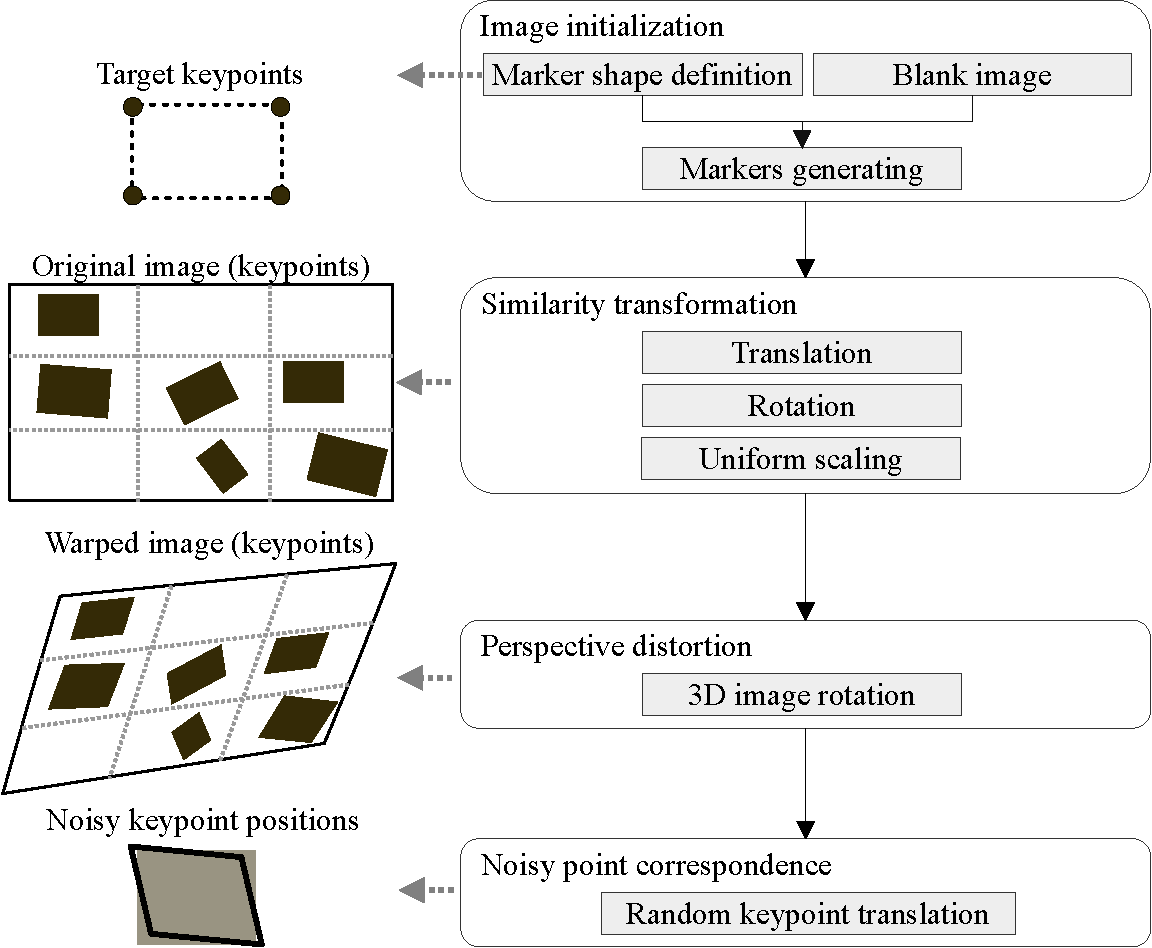
\includegraphics[width=0.7\linewidth]{figures/homography/dataset_generating.pdf}
    \caption[Description of creation of test scenarios]{Description of how each one of $t$ test instances in a specific test scenario is created. The input is a blank $w \times h$ image over which $m$ markers are initialized in a uniform grid, which produces the original marker keypoints. Depending on the test scenario, a particular subset of similarity transformations is applied to the entire image. Subsequently, warped keypoints are modified by random noise to simulate noisy point correspondence.}
    \label{fig:DatasetGenerating}
\end{figure}
% ------------------------------------------------------------------------------

% ##############################################################################
\subsection{Evaluation Methodology}
\label{ssec:evaluation_methodology}

\subsubsection{Error Computation}
\label{sssec:error_computation}

\def\warpedpix{\vect{w}}
\def\origpix{\vect{g}}

The accuracy of the developed method was evaluated by measuring the reprojection error using the Euclidean distance between the original and the rectified pixel positions. To obtain an error over the entire image, we computed the error for each pixel. Specifically, let $w$ and $h$ be the width and height of the image, respectively. The $3$D rotation of a point in the image around the image center that produces perspective distortion is represented by $\func{\varphi}{\cdot}$. Let $\subsup{\origpix}{i,j}{T} = \sbrackets{j, i, 1}$ be the original (ground-truth) pixel position at the $i$-th row and $j$-th column, and let $\warpedpix_{i, j} = \func{\varphi}{\origpix_{i, j}}$ be the analogically defined warped pixel position, for $i = 1, \dots, h, j = 1, \dots, w$. We then compute the $2$D reprojection error grid (a $h \times w$ matrix) for the given homography $\H$ as
\begin{equation}
    \label{eq:reprojection_error_grid}
    \boldsymbol{\xi}_{wh} =
    \begin{bmatrix}
        \func{e}{\warpedpix_{1, 1}, \origpix_{1, 1}} & \dots & \func{e}{\warpedpix_{1, w}, \origpix_{1, w}} \\
        \dots                                        & \dots & \dots                                        \\
        \func{e}{\warpedpix_{h, 1}, \origpix_{h, 1}} & \dots & \func{e}{\warpedpix_{h, w}, \origpix_{h, w}}
    \end{bmatrix},
\end{equation}
where
\begin{equation}
    \func{e}{\warpedpix, \origpix} = \euclnorm{\H \warpedpix - \origpix}.
\end{equation}
To simply express the reprojection error as a single number for the whole image, we adopted an arithmetic mean of all the values in the error grid above, so
\begin{equation}
    \label{eq:ReprojectionErrorSingle}
    \xi_{\text{reproj}} =
    \frac{1}{wh}
    \sum_{i = 1}^{h}
    \sum_{j = 1}^{w}
    \func{e}{\warpedpix_{i, j}, \origpix_{i, j}}.
\end{equation}

\subsubsection{Evaluation Algorithm}
\label{sssec:EvaluationAlgorithm}

On the input, there are $m$ markers (\sectionstr{}~\ref{ssec:HomographyDatasetCreation}) and thus an $m$-to-$1$ point correspondence. Each marker, by definition, provides a unique homography. Therefore, the aim is to quantify the relative improvement in the reprojection error over the baseline when the $k$-th ranked homography is used for rectification. Even though we are primarily concerned only with the single, top-performing homography, we evaluate the entire ranking to demonstrate its stable behavior.

We evaluated our homography ranking in terms of reprojection error improvements against the existing approaches based on the isolated homography estimation represented by implementation from the OpenCV~\cite{bradski2008learning} library. Since our method provides a ranking, we compare our performance against a random marker selection based on uniform probability distribution. We refer to this performance as the ``baseline''; an unbiased marker selection. In practice, the user would rely on ``educated guess'' when predicting which marker could potentially be the best one to use. To obtain the aforementioned baseline, we evaluated the reprojection error \ref{eq:ReprojectionErrorSingle} for each marker in isolation and computed the arithmetic mean of these values. When we executed our proposed algorithm, we got the full ordering of markers by their score value computed using the proposed criterion \ref{eq:HomographyScoreFunction}. We expected that if the first marker were used to rectify the image, then the reprojection error would be minimal (and lower than the baseline error). If any subsequent marker in the given order were used instead, the reprojection error would increase.

We computed the relative improvement in \% for each $k$-th homography according to the baseline performance. Each test scenario was evaluated one by one. For each test instance, we obtained a $k$-dimensional vector where its elements represented a percentual improvement at each $k$-th position. We represented our data as a $t \times k$ matrix, where $t$ was the number of test instances. We treated each column independently to compute the statistics. The details of our evaluation algorithm are described in Algorithm~\ref{alg:EvaluationAlgorithm}. For simplicity, we show an evaluation of just a single instance.

\def\meanerrs{\boldsymbol{e}}
\def\errdiffs{\boldsymbol{p}}
\def\arracc{\left[ \right]}

\begin{algorithm}[t]
    \caption{Evaluation Algorithm}
    \label{alg:EvaluationAlgorithm}
    \begin{algorithmic}[1]
        \State $\hmatrices, \sortres \gets $ \Call{rankhomographies}{\ }
        \Comment{Algorithm~\ref{alg:HomographyRanking}}

        \State $e_b \gets 0$
        \Comment{baseline}

        \State $\meanerrs \gets \arraydef \left[ m \right]$
        \Comment{reprojection errors}

        \State $\errdiffs \gets \arraydef \left[ m \right]$
        \Comment{relative improvements}

        \For{$i \gets 1, \dots , m$}
        \State $\meanerrs \left[ i \right] \gets $ $\xi_{\text{reproj}}$
        \Comment{\eqstr{}~\ref{eq:ReprojectionErrorSingle}}

        \State $e_b \gets e_b + \meanerrs \left[ i \right]$
        \EndFor

        \State $e_b \gets e_b / m$
        \Comment{mean reprojection error}

        \For{$i \gets 1, \dots , m$}
        \State $k \gets \sortres \left[ i \right]$
        \Comment{position of $i$-th best homography}

        \State $\errdiffs \left[ i \right] \gets \rbrackets{e_b - \meanerrs \left[ k \right]} / e_b$
        \Comment{relative improvement}
        \EndFor

        \State \Return $\errdiffs$
    \end{algorithmic}
\end{algorithm}

% ##############################################################################
\subsection{Experimental Results}
\label{ssec:EvaluationResults}

\figstr{}~\ref{fig:HeatmapsBestWorst} shows how the reprojection error varies with respect to the marker position. We can see that the marker position can be deduced by looking at the heatmap representing the pixel-wise reprojection error over the image. The transformation achieves the best accuracy in the marker neighborhood and steadily decreases for more distant pixels. However, not all markers are subjected to the same pattern of error variation. This observation was the core motivation for our solution. We aim to choose the marker that minimizes the pixel-wise reprojection error within the region of the image that is as broad as possible. That is why we evaluate our method by computing the reprojection error over each pixel, not just the keypoints.

All tested scenarios depict similar trends as shown on the plots in \figstr{}~\ref{fig:SimilarityTransformInfluence}, \figstr{}~\ref{fig:NoiseInfluence}, \figstr{}~\ref{fig:ShapeInfluence} and in \figstr{}~\ref{fig:NMarkersInfluence}. The box plots extend from the lower to upper quartile values, with the thin and thick lines representing the median and mean, respectively. The plots discussed further show relative improvements over the baseline OpenCV~\cite{bradski2008learning} method. We evaluated relative improvements for the sake of interpretability. For better comprehension, we suggest to see \tablestr{}~\ref{tab:TestScenariosResults}. It contains individual test scenarios and their corresponding top performances in percents. Conversely, the reprojection error in absolute terms is difficult to interpret without additional context. Nevertheless, to highlight the differences in reprojection errors we also provide absolute values in \tablestr{}~\ref{tab:TestScenariosResults}. The presence of noise shifted the errors by multiple magnitudes, but still preserved the pattern of distribution.

\subsubsection{Influence of Similarity Transformations}

In this test scenario, we tested in isolation each allowed similarity transformation, i.e., translation, rotation, and uniform scaling. \figstr{}~\ref{fig:SimilarityTransformInfluence} demonstrates that the relative improvement was circa equal in all situations. Besides, we show that the proposed method is practically invariant to similarity transformations allowing the markers to be in arbitrary positions in a plane. When all similarity transformations were utilized, our method performed even better, showing its stability and robustness.

\def\boxplotimgwidth{0.75\linewidth}

% ------------------------------------------------------------------------------
\begin{figure}[t]
    \centering
    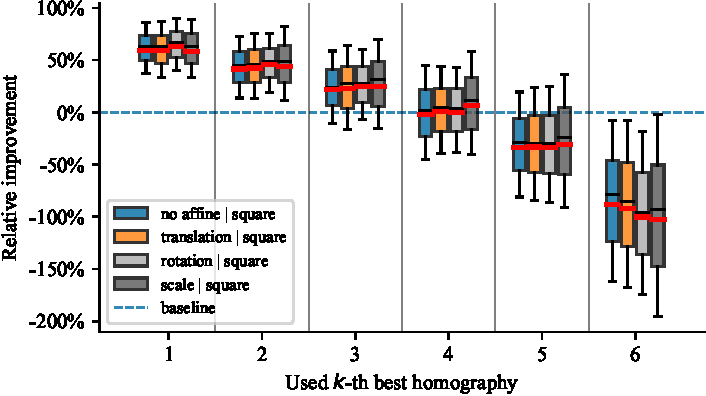
\includegraphics[width=\boxplotimgwidth]{figures/homography/similarity_transform_influence.pdf}
    \caption[Influence of similarity transformation]{Influence of similarity transformation on the reprojection error.}
    \label{fig:SimilarityTransformInfluence}
\end{figure}
% ------------------------------------------------------------------------------

\subsubsection{Influence of Noise}

In \figstr{}~\ref{fig:NoiseInfluence}, we can see the effect of noisy point correspondence that simulated inaccurate keypoint detection. The ranking method preserved the trend of the relative improvement in presence of noise. Absolute reprojection error demonstrated that unless noise was present, the errors varied on sub-pixel levels, so they were practically zero.

% ------------------------------------------------------------------------------
\begin{figure}[t]
    \centering
    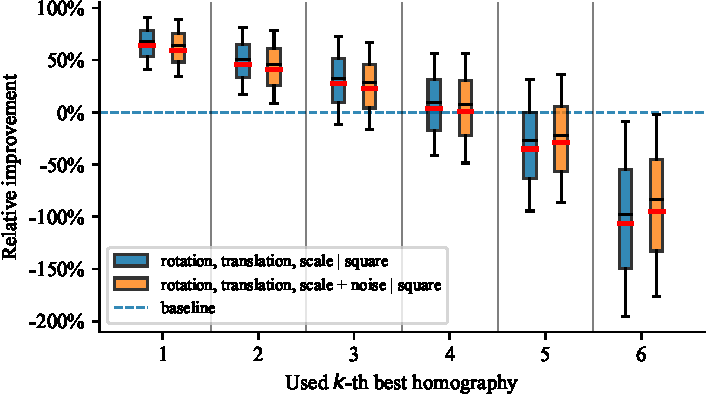
\includegraphics[width=\boxplotimgwidth]{figures/homography/noise_influence.pdf}
    \caption[Influence of noise]{Influence of noise applied to the warped keypoints representing a noisy point correspondence.}
    \label{fig:NoiseInfluence}
\end{figure}
% ------------------------------------------------------------------------------

\subsubsection{Influence of Variable Shapes}

We expected that the relative improvement of our method should be invariant to variable shapes as long as they were similar. \figstr{}~\ref{fig:ShapeInfluence} demonstrates that with an increasing number of keypoints our method consistently preserved its capabilities. Introducing more complicated shapes than just rectangles did not exacerbate the outcome of the algorithm.

% ------------------------------------------------------------------------------
\begin{figure}[t]
    \centering
    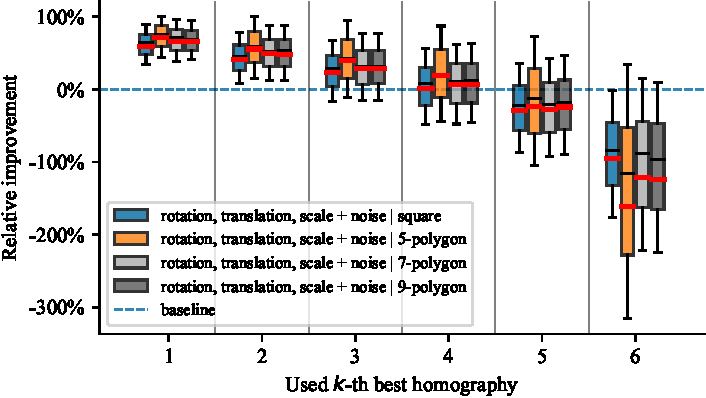
\includegraphics[width=\boxplotimgwidth]{figures/homography/shape_influence.pdf}
    \caption[Influence of marker shape]{Results for different marker shapes.}
    \label{fig:ShapeInfluence}
\end{figure}
% ------------------------------------------------------------------------------

\subsubsection{Influence of Number of Markers}

We tested a variable number of markers to demonstrate that our method preserved its improvement. \figstr{}~\ref{fig:NMarkersInfluence} shows that the greater the set of markers, the better the relative improvement of our method. Even when we used just three markers, the proposed method achieved a $46.91$\% median relative improvement.
While it is beneficial to use a larger number of markers, we believe that the improvement we can obtain from an increasing number of markers has a logarithmic trend. On the extreme side, if we used only one marker, there would be no improvement since there would be only one homography to choose from.

\begin{figure*}[t]
    \centering
    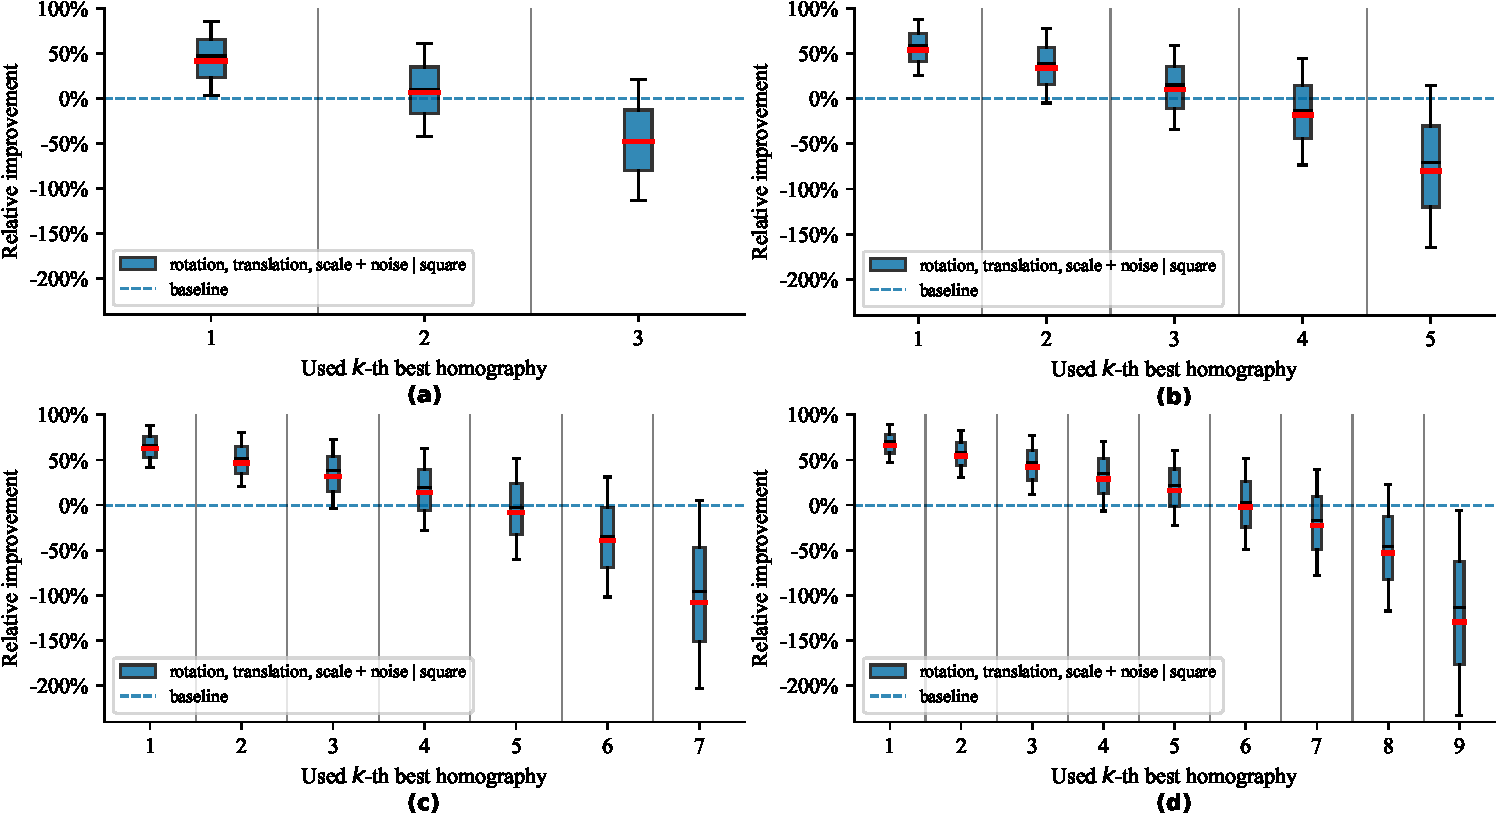
\includegraphics[width=\linewidth]{figures/homography/n_markers_influence.pdf}
    \caption[Influence of number of markers]{Influence of different number of markers on reprojection error. We experimented with \imgpartdesc{a} three, \imgpartdesc{b} five, \imgpartdesc{c} seven, and \imgpartdesc{d} nine markers.}
    \label{fig:NMarkersInfluence}
\end{figure*}

\def\tblsccolw{0.06}
\def\tblrscolw{0.08}
\begin{table*}[t]
    \caption[Description of syntehtic dataset scenarios]{Description of test scenarios in our synthetic dataset with corresponding settings and results for the top-ranked homography. One row represents one test scenario. Four visually separated groups (from top to bottom) are related to experiments shown in \figstr{}~\ref{fig:SimilarityTransformInfluence}~-~\ref{fig:NMarkersInfluence}.}
    \label{tab:TestScenariosResults}
    \setlength{\tabcolsep}{3pt}
    \begin{center}
        \footnotesize
        \begin{tabular}{p{\tblsccolw\linewidth}p{0.03\linewidth}p{\tblsccolw\linewidth}p{\tblsccolw\linewidth}p{\tblsccolw\linewidth}p{\tblsccolw\linewidth}|p{\tblrscolw\linewidth}p{\tblrscolw\linewidth}p{\tblrscolw\linewidth}p{\tblrscolw\linewidth}p{\tblrscolw\linewidth}p{\tblrscolw\linewidth}}
            \toprule
            \multirow{2}{2pt}{\textbf{shape}}  &
            \multirow{2}{2pt}{\textbf{\#}}     &
            \multirow{2}{2pt}{\textbf{trans.}} &
            \multirow{2}{2pt}{\textbf{rot.}}   &
            \multirow{2}{2pt}{\textbf{scale}}  &
            \multirow{2}{2pt}{\textbf{noise}}  & \multicolumn{3}{l}{\textbf{relative improvement}} & \multicolumn{3}{l}{\textbf{absolute improvement}}                                                                                                      \\
                                               &                                                   &                                                   &     &     &     & \textbf{median} & \textbf{mean} & \textbf{stdev} &
            \textbf{median}                    & \textbf{mean}                                     & \textbf{stdev}                                                                                                                                         \\
            \midrule
            square                             & 6                                                 & no                                                & no  & no  & no  & 62.80\%         & 59.63\%       & 19.64\%        & 0.0003  & 0.0003   & 0.0001   \\
            square                             & 6                                                 & yes                                               & no  & no  & no  & 62.65\%         & 59.00\%       & 19.72\%        & 0.0003  & 0.0003   & 0.0001   \\
            square                             & 6                                                 & no                                                & yes & no  & no  & 66.42\%         & 63.17\%       & 19.11\%        & 0.0004  & 0.0004   & 0.0002   \\
            square                             & 6                                                 & no                                                & no  & yes & no  & 63.38\%         & 58.51\%       & 23.97\%        & 0.0002  & 0.0003   & 0.0002   \\
            \midrule
            square                             & 6                                                 & yes                                               & yes & yes & no  & 67.82\%         & 63.66\%       & 20.30\%        & 0.0004  & 0.0004   & 0.0002   \\
            square                             & 6                                                 & yes                                               & yes & yes & yes & 64.11\%         & 59.26\%       & 22.12\%        & 22.0781 & 24.3177  & 15.0085  \\
            \midrule
            5-poly                             & 6                                                 & yes                                               & yes & yes & yes & 74.67\%         & 71.19\%       & 21.98\%        & 69.5553 & 336.2653 & 685.7427 \\
            7-poly                             & 6                                                 & yes                                               & yes & yes & yes & 71.02\%         & 65.63\%       & 22.99\%        & 46.7939 & 135.6574 & 395.7526 \\
            9-poly                             & 6                                                 & yes                                               & yes & yes & yes & 68.97\%         & 65.57\%       & 21.98\%        & 44.9763 & 115.1219 & 309.2720 \\
            \midrule
            square                             & 3                                                 & yes                                               & yes & yes & yes & 46.91\%         & 41.36\%       & 31.58\%        & 14.7750 & 18.1155  & 20.6746  \\
            square                             & 5                                                 & yes                                               & yes & yes & yes & 59.03\%         & 53.91\%       & 24.56\%        & 19.7629 & 22.5333  & 16.0080  \\
            square                             & 7                                                 & yes                                               & yes & yes & yes & 66.19\%         & 62.41\%       & 19.98\%        & 23.8768 & 27.1364  & 32.2853  \\
            square                             & 9                                                 & yes                                               & yes & yes & yes & 69.86\%         & 66.09\%       & 18.18\%        & 25.6645 & 26.6838  & 11.6975  \\
            \bottomrule
        \end{tabular}
    \end{center}
\end{table*}